% 图 8.26 有机铁磁体 p-NPNN（对硝基苯基硝酮氮氧自由基）分子骨架式
\documentclass[tikz,border=5pt]{standalone}
\usetikzlibrary{arrows.meta}
\usepackage{amsmath}
\usepackage{bm}
\usepackage{fontspec}
\setmainfont{Times New Roman}
\begin{document}
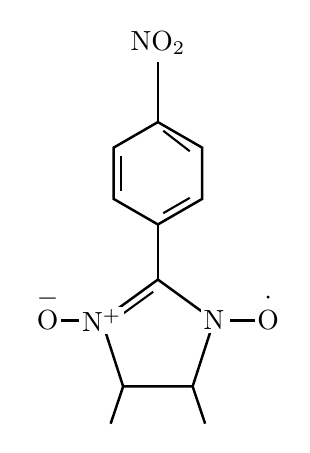
\begin{tikzpicture}[line width=0.9pt,>=Stealth]
% ---------- bonds ----------
% NO2 substituent
\node[fill=white,inner sep=1.5pt] at (0,4.5) {$\mathrm{NO}_2$};
\draw (0,4.26) -- (0,3.5);
% benzene ring
\draw (0,3.5) -- (0.563,3.175) -- (0.563,2.525) -- (0,2.2)
      -- (-0.563,2.525) -- (-0.563,3.175) -- cycle;
% Kekule double bonds (inner offset lines)
\draw[line width=0.75] (0.068,3.390) -- (0.405,3.130);
\draw[line width=0.75] (0.405,2.538) -- (0.068,2.343);
\draw[line width=0.75] (-0.473,2.630) -- (-0.473,3.070);
% phenyl -> nitronyl nitroxide ring
\draw (0,2.2) -- (0,1.5);
% five-membered ring: C(0,1.5), N(0.713,0.982), C(0.441,0.143),
%                     C(-0.441,0.143), N(-0.713,0.982)
\draw (0,1.5) -- (0.713,0.982) -- (0.441,0.143) -- (-0.441,0.143)
      -- (-0.713,0.982) -- cycle;
% C=N+ double bond (inner offset line)
\draw[line width=0.75] (-0.060,1.345) -- (-0.547,0.991);
% N+ -- O- (left)
\draw (-0.92,0.982) -- (-1.26,0.982);
% N -- O. (right)
\draw (0.92,0.982) -- (1.26,0.982);
% methyl stubs on the two ring carbons
\draw (-0.441,0.143) -- (-0.60,-0.33);
\draw (0.441,0.143) -- (0.60,-0.33);
% ---------- atom labels ----------
\node[fill=white,inner sep=1pt] at (-0.713,0.982) {$\mathrm{N}^{+}$};
\node[fill=white,inner sep=1pt] at (0.713,0.982) {$\mathrm{N}$};
\node[fill=white,inner sep=1pt] at (-1.40,0.982) {$\mathrm{O}$};
\node at (-1.40,1.26) {$-$};
\node[fill=white,inner sep=1pt] at (1.40,0.982) {$\mathrm{O}$};
\node at (1.40,1.26) {$\cdot$};
\end{tikzpicture}
\end{document}
